\customchapter{Architecture Concepts}

\section{Bus concept}

\subsection{Introduction to AXI4-Lite Bus}
The AXI4-Lite interface facilitates communication between the programmable logic (PL) peripheral device and the software running on the processing system (PS). Unlike the standard AXI bus, AXI4-Lite is tailored for simplicity, mainly focusing on the control and monitoring of IP blocks in the ZYNQ device, establishing a connection between ARM and FPGA components.

\subsection{AXI4-Lite Functionality}
AXI4-Lite is designed to handle 32-bit read-and-write data transfers. However, it differs from the standard AXI as it does not supporting variable bus width or cache operations. Each read or write operation allows only a single 32-bit data transfer. Its primary purpose lies in controlling and monitoring IP blocks, serving as an effective communication bridge between the ARM and FPGA elements.
\subsection{AXI4-Lite Channels}
The AXI bus structure incorporates distinct channels for read and write transactions, enabling semi-independent progression. These channels include Read Address, Read Data, Write Address, Write Data, and Write Response. Each channel is equipped with handshaking signals to manage operations.
\subsection{Read and Write Channels} 
\begin{itemize}
    \item 	Read Address and Read Data Channels: Responsible for moving data from the slave to the master.
    \item 	Write Address, Write Data, and Write Response Channels: Transfer data from the master to the slave.
    \item 	Concurrent read and write transactions are supported without interference.
    \item 	Handshaking signals, such as READY and VALID, are unique to each channel, allowing for efficient coordination.
\end{itemize}

\subsection{ Concurrent Transactions}
Figure 4.2 illustrates the overall flow of AXI4-Lite bus transactions, highlighting the concurrent nature of read and write operations. This flexibility ensures that the Write Address and Write Data channels can operate simultaneously or sequentially, with additional considerations for a second write address (A2) before the completion of the previous write cycle (A0).
\subsection{AXI4-Lite IP Interface (IPIF)} 
The AXI4-Lite IP Interface (IPIF) is an integral part of the Xilinx family, providing a bidirectional interface between a user Intellectual Property (IP) core and the AXI interconnect. Its purpose is to simplify the connection between ARM AXI and user IP cores, streamlining the management of different addresses.

\newpage

\begin{figure}[h] % Use the 'h' option to try to place the image "here"
  \centering
  \setlength{\abovecaptionskip}{0pt} % Reduce space above the caption
  \setlength{\belowcaptionskip}{0pt} % Adjust space below the caption
  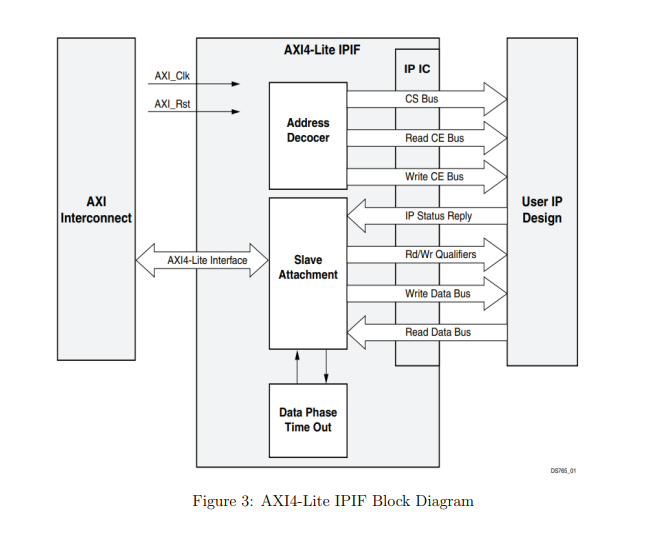
\includegraphics[width=.7\textwidth]{Image/AXI.png} % Replace 'your-image.png' with the actual file name
  \caption{AXI transaction}
  \label{Figure 1 : RISC-V instruction formats}
\end{figure}


\subsection{Features of AXI4-Lite IPIF} 
\begin{itemize}
    \item 	32-bit Slave Configuration: Supports a 32-bit slave configuration for effective data handling.
    \item 	Read and Write Data Transfers: Facilitates read and write data transfers of 32-bit width.
    \item   Multiple Address Ranges: Supports multiple address ranges for versatile IP core integration.
    \item 	Read Priority Over Write: Prioritizes read operations over write operations.
    \item 	Address Space Handling: Reads to holes in the address space returns 0x00000000, and writes to holes after the register map is ignored and responds with an OKAY response.
\end{itemize}




\section{System control concept}

The entire system is controlled by a processing system (PS). In this case, the chosen PS is an ARM Cortex A-9 processor. The main significance of the processor is to control the functionalities of the peripherals interfaced with it. In this case, the PS controls the peripherals deployed on the programmable Logic (PL) of SoC over the AXI-lite bus after establishing a successful handshake mechanism. 
\vspace{2mm}

The custom IP has 32x 32-bit registers. This IP is memory-mapped with the ARM core through an AXI-lite bus. The PS can read and write data into a register file via AXI bus using the base address of the peripheral. The Xilinx design platform is vast and provides an IDE to develop custom drives and firmware for our custom IPs. Vitis is one such IDE where the custom IP which is designed in the Vivado tool can be exported as an HDL wrapper for further application development and testing.



% ARM CORE Refshuffled from here


\newpage

\section{Clock system} 

The Zynq-7000 SoC (System on Chip) from Xilinx integrates both a Processing System (PS) and programmable logic (PL). The PS includes ARM Cortex-A9 processors, and the clocking architecture involves several clock sources. Here are some of the key clock sources in the Zynq-7000:

\begin{itemize} \item \textbf{PS Clocks:}


     ARM Cortex-A9 Clocks (CPU\_CLK): The ARM Cortex-A9 processors in the PS have their own clocks. Maximum possible clock frequency of ARM Cortex-A9 is 866MHz.
\end{itemize}


 \begin{itemize}
     \item \textbf{PL Clocks:}
     

     FCLKs (Fabric Clocks): These clocks are generated by the Clock Management Unit (CMU) in the PS and are typically used to clock logic within the programmable fabric (PL). FCLK\_CLK0 is an example, but there can be multiple FCLKs available. The clock frequency of  FCLK\_CLK0 is 100MHz. This is the configured PL clock frequency in our design, hence all the custom logic elements within the PL section will receive this clock frequency.
 \end{itemize}
\section{Debug Concept}

The Test Access Port (TAP) controller is a fundamental component of the Joint Test Action Group (JTAG) interface, which is used for testing and debugging digital electronic devices, such as integrated circuits (ICs), printed circuit boards (PCBs), and other hardware systems. The TAP controller manages the communication and control between a JTAG-compliant device and an external test or debugging tool.


\vspace{2mm}
The designed system can be further tested in detail with the help of a TAP controller based on the IEEE 1149.1 standard. The implementation of the TAP controller is explained in a further section in great detail.



\section{RISC-V Instruction Set Architecture}
The custom register peripheral needs to be compatible with the RISC-V ISA. Based on the ideas of reduced instruction set computing (RISC), RISC-V is an open standard instruction set architecture (ISA). Since RISC-V is an open standard, anyone can implement their own RISC-V processors without having to pay license costs because the architecture's specifications are made available to the public. Because RISC-V instructions have a set length (usually 32 bits), pipelining and decoding in processor designs are made easier. Because RISC-V has a load-store architecture, load and store instructions are the only ways to access memory and all data processing instructions function on registers. 
\newpage
\begin{figure}[h] % Use the 'h' option to try to place the image "here"
  \centering
  \setlength{\abovecaptionskip}{0pt} % Reduce space above the caption
  \setlength{\belowcaptionskip}{0pt} % Adjust space below the caption
  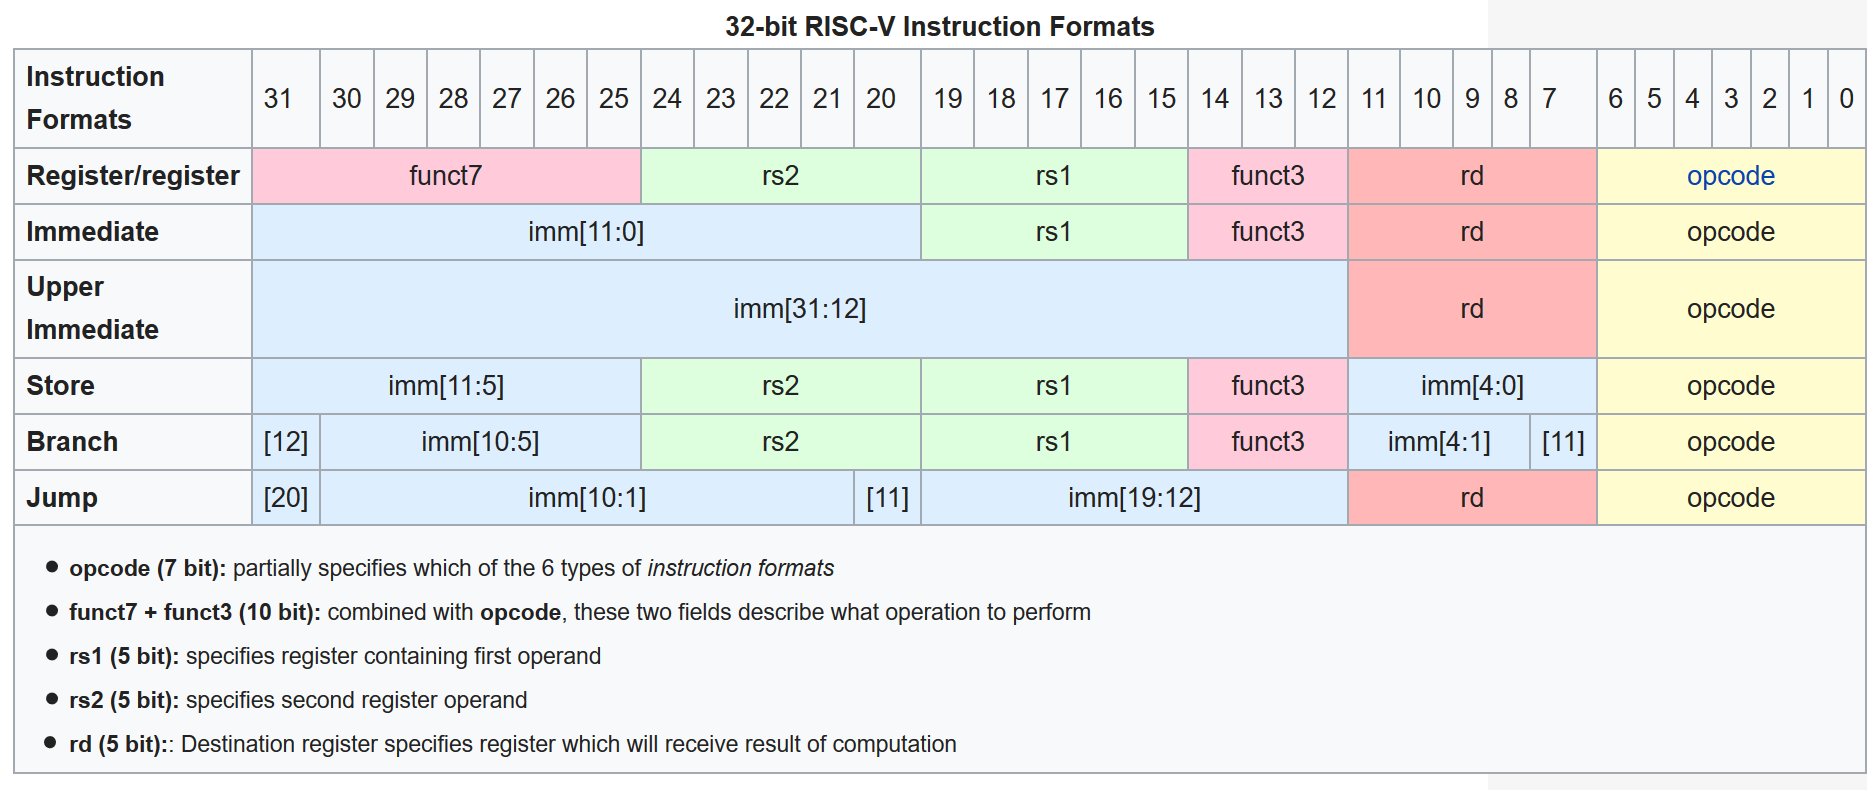
\includegraphics[width=1.0\textwidth]{Image/RISC V.png} % Replace 'your-image.png' with the actual file name
  \caption{RISC-V instruction formats}
  \label{Figure 1 : RISC-V instruction formats}
\end{figure}

A variety of instruction forms are available for RISC-V, including I-type (immediate value operations), S-type (store instructions), B-type (branch instructions), J-type (jump instructions), R-type (register-register operations), the figure 7 depicts the same. Multiple integer and floating-point register sets are provided by RISC-V and can be utilized for a variety of applications. This adaptability helps in managing various application domains and data kinds.

